\section{Implementation}
\label{sec:implementation}

Web application development framework \textit{Django}~\cite{django}, Web API toolkit \textit{Django REST Framework} (DRF)~\cite{drf} and Python~\cite{python} library \textit{django-filter}~\cite{django-filter} are used to operate \boatvtwo.
PostgreSQL~\cite{psql} is used to provide a database for the server-side applications of the software.
During the implementation phase, decisions regarding models of the database have been directed towards the UI utilizing the API for database queries and searches.
The models reflect the \ud\ format of sentences and annotations are saved as fields of word lines.

All the pages of the tool have been supported by Bootstrap~\cite{bootstrap}.
The annotation page has most of the functionalities of \boatvone.
Entries are validated and errors are displayed on the annotation page for annotators to see invalid edits in real time, according to the \ud\ framework~\cite{UD} and the language provided.

Python library \textit{spa\textsc{C}y}~\cite{spacy} is used to provide linear dependency graphs.
Another JavaScript-based linear dependency graph~\cite{spyssalo} making use of \textit{brat}~\cite{brat} is used to provide graphs as well.
An annotator's preference regarding this may vary, thus, giving them visualization options is important.

\begin{figure}[tbh]
    \centering
    %\frame{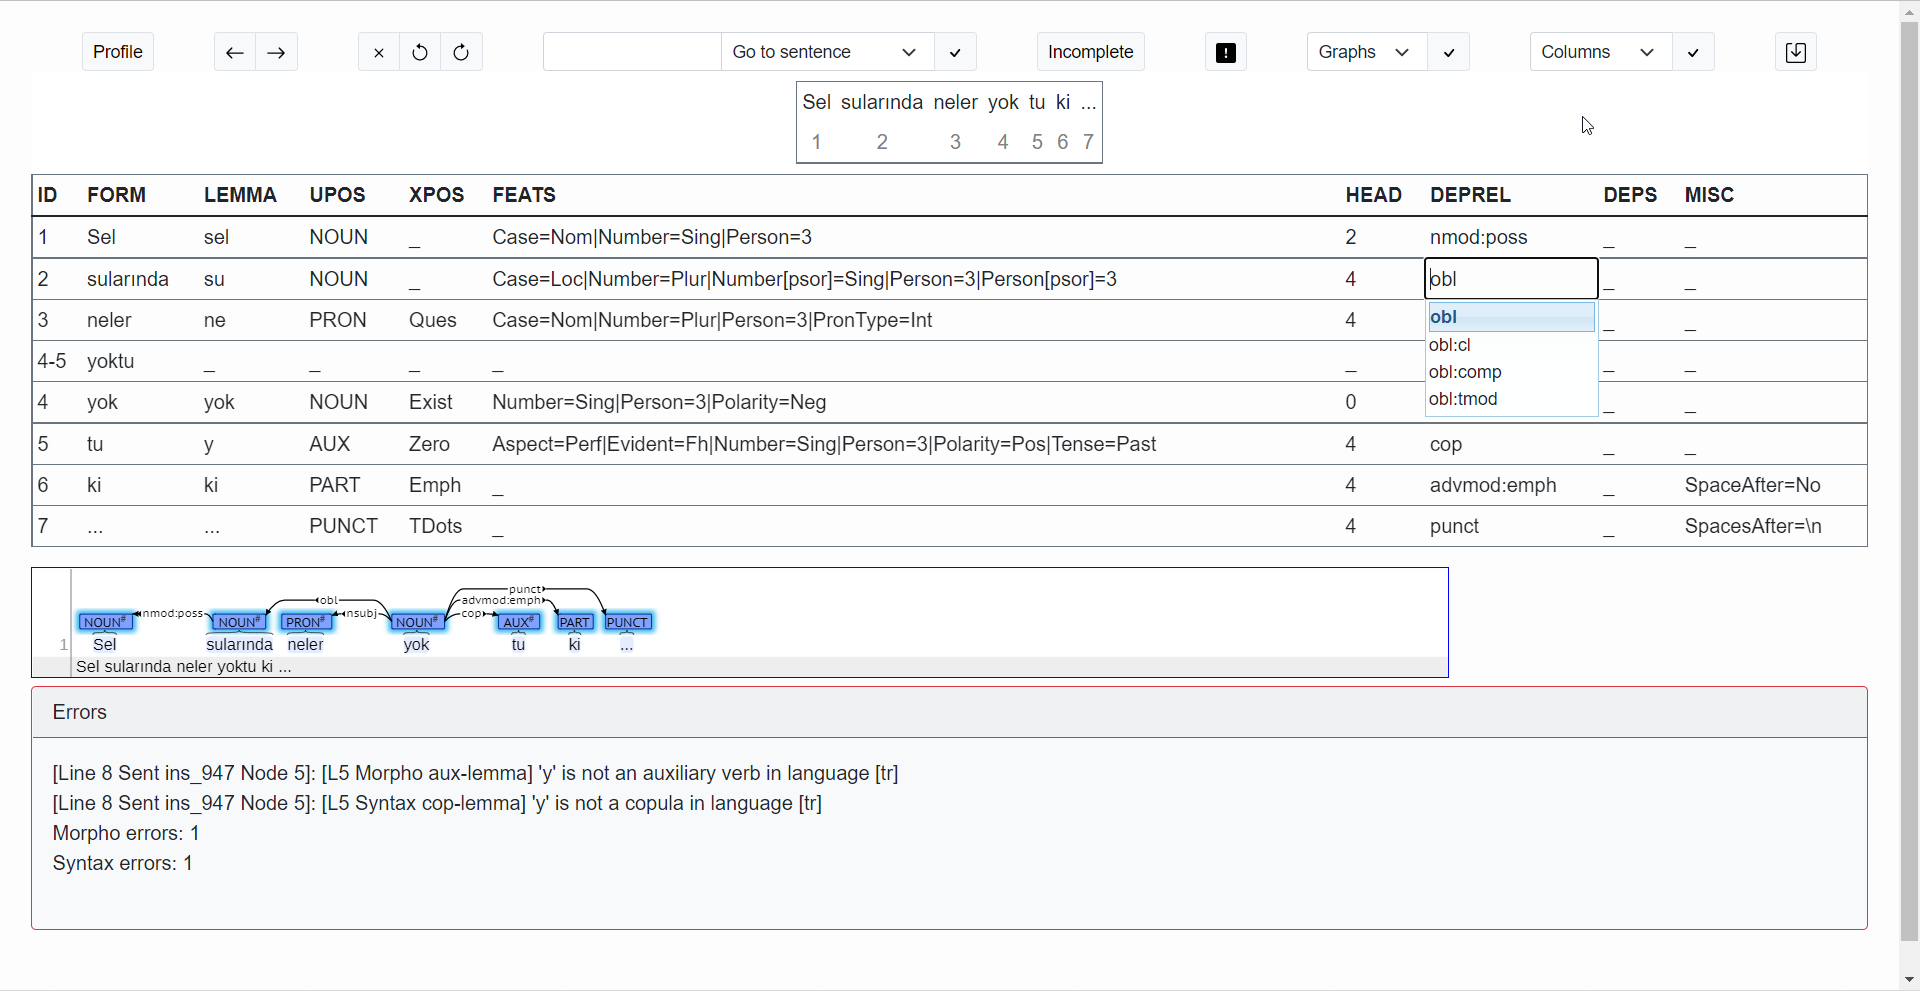
\includegraphics[width=1\textwidth]{figures/sample-annotation.png}}
         \tcbox[left=0mm,right=0mm,top=0mm,bottom=0mm,boxsep=1pt,arc=0mm,boxrule=0.5pt,colframe=black,sharp corners]
    {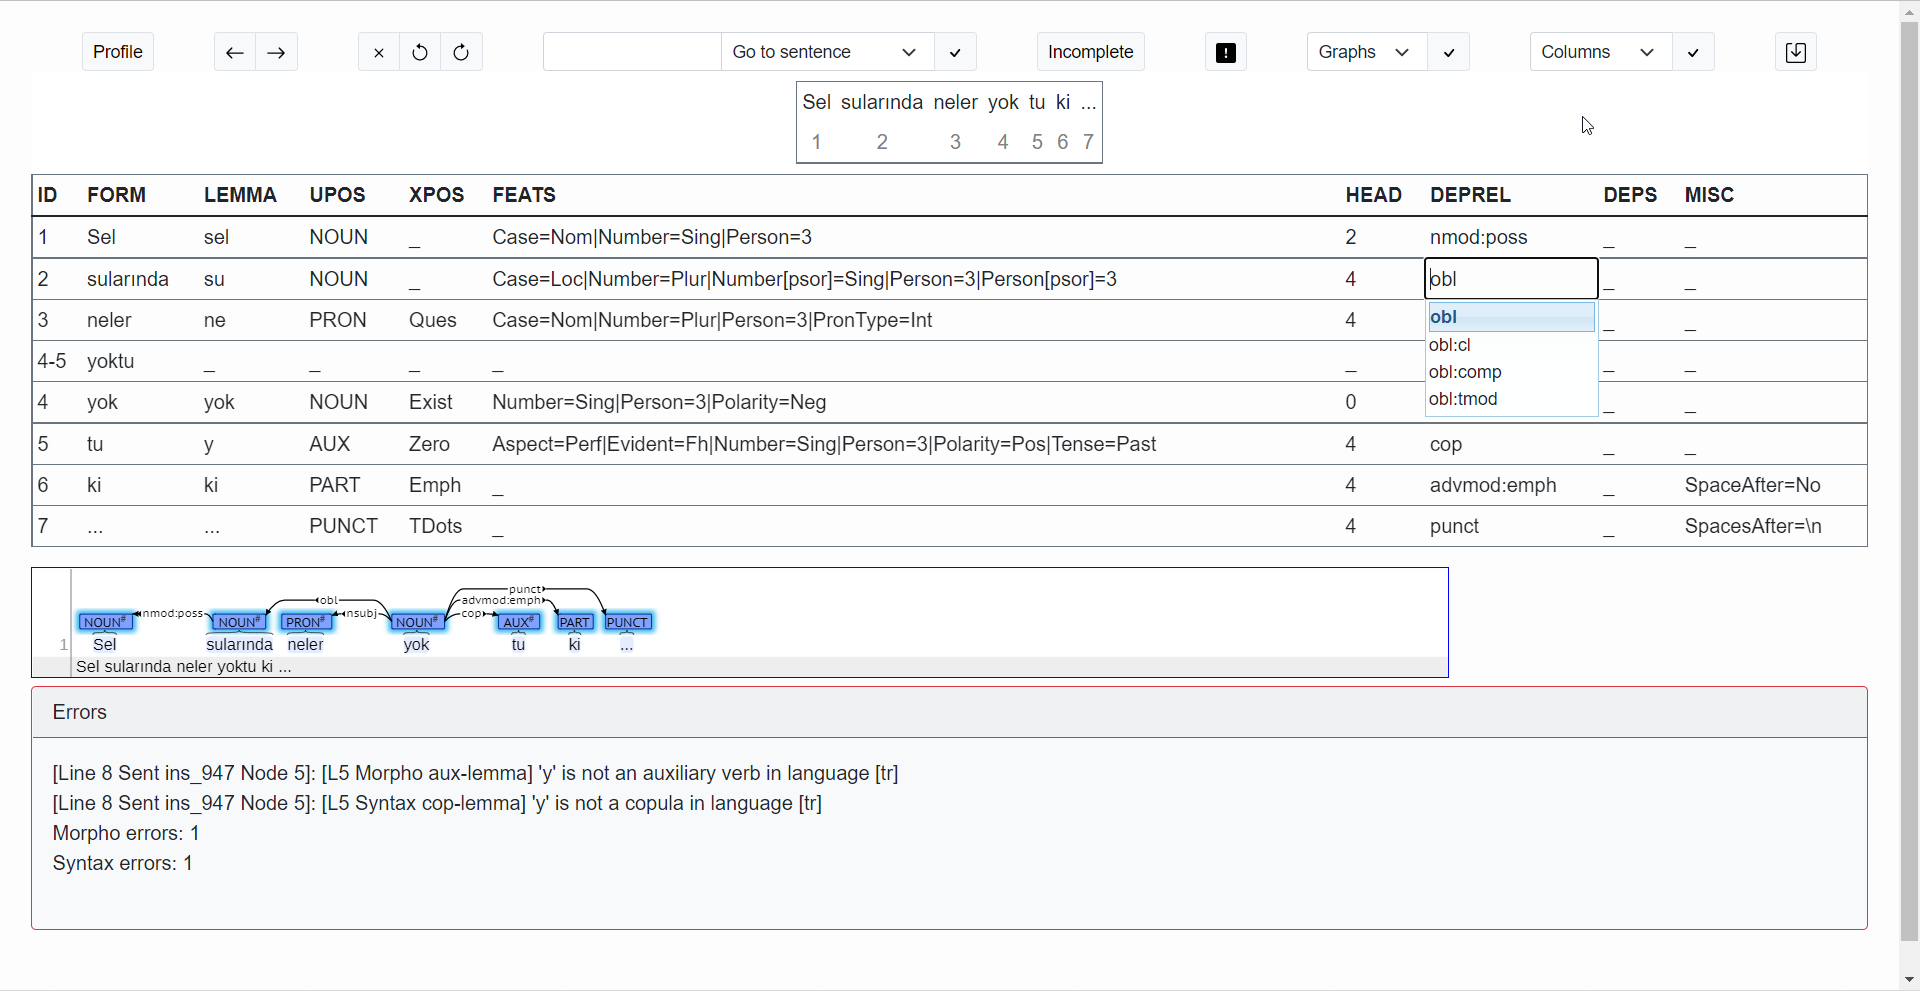
\includegraphics[width=1\textwidth]{figures/sample-annotation.png}}
    \caption{The annotation screen captured while the sentence ``Sel sularında neler yoktu ki...'' is being annotated. The \deprel\ tag for the \form\ ``sularında'' is being annotated by selecting among the valid alternatives that appear in the pop-up. Selections can be made with use of arrow keys.}
    \label{fig:anno-fig}
\end{figure}

\subsection{Features}
\label{sec:features}

There are many new features and improvements in this tool, as well as most of the functionality of \boatvone.

\begin{itemize}[before=\normalfont, font=\itshape, align=left]
    \item[Treebanks:]
        Multiple treebanks, with each one having its own sets of sentences, can be created in a single deployment.
        When uploading a file, a treebank is selected.

    \item[Loading files:]
        Instead of loading a dataset file before every annotation session, a \conllu\ file is uploaded to the database.
        The file is rejected if incorrectly formatted, otherwise uploaded to the database.
        This way, other annotators working with the same treebank don't have to provide the same file.

    \item[Annotation view:]
        The annotation page is very similar to the one on \boatvone~\cite{trk2020resources}, as seen in Figure~\ref{fig:anno-fig}.
        There is an annotation table for annotating fields in word lines of sentences.
        It also includes a dependency graph and an error card, both of which are in sync with the edits done on the table cells.
        Three different dependency graph representations are provided in this tool.
        Two of the graphs, which are both horizontal and linear, have been selected due to space considerations.
        The error card displays errors for the current annotation, validating it via the UD validation script.

    \item[Network-enabled search:]
        An important feature in this version is the ability to cross-check annotations by implementing a network for annotators where they can review the annotations done by other annotators.
        This can be helpful and a learning experience for annotators.

        For example, the annotator of the \bountreebank was annotating a sentence with a Zodiac sign noun.
        Not being sure of how to annotate its \upos\ tag, she searched the \conllu\ file manually for similar cases and encountered two different values with which nouns of Zodiac signs were annotated previously.
        Besides not helping how to choose a \upos\ tag, this raises a consistency issue within the treebank as well.
        This task could have been handled by a search of the database.
        We provide a search page and an API in this tool with which treebanks can be searched by \ud\ tags.

        Another example could be given by the various \textit{-ki} morphemes in Turkish.
        In the sentence ``Evdeki halılar yıkandı.'' (\textit{The rugs at home were washed.}), the \textit{-ki} acts as an adjectivizer.
        However, in ``Benim halılarım yün, Ayşeninkiler sentetik.'' (\textit{My rugs are woolen. Ayşe's are synthetic.}), it is pronominal.
        An annotator might not recall how a specific \textit{-ki} morpheme should be annotated, which can be remedied with a simple search.
        Annotators have informed us that such cases occur frequently when annotating MRLs.

        The inter-annotator agreement allows us to see some anomalies in the Turkish part of the \ud\ framework.
        For example, if a sentence were annotated a way by many annotators but the \ud\ validation script were finding it invalid, this might indicate the validation were lacking in this respect of the Turkish language.

    \item[Annotation status:]
        There are 3 annotation statuses ("Incomplete", "Draft" and "Complete") and they are cycled through by the annotator in the annotation view.
        Status of an annotation is also shown in the search view, helping to select an appropriate case.
        There is another view where completed, drafted or incomplete annotations can be listed.

\end{itemize}
